% !TEX root = ../partial-sdm.tex

\section{Results (iv): Supervised classification application}

Supervised classification problem consists of categorize data into groups after seeing some samples from each group. First, it is presented pieces of data with their categories. The algorithm learns from these data, which is known as learning phase. Then, new pieces of data are presented and the algorithm must classify them into the already known groups. It is named supervised because  the algorithm will not create the groups itself. It will learn the groups from during the learning phase, in which the groups have already been defined and the pieces of data have already been classified into them.

Although this problem has already been studied (REF), our intention here is to show that a pure SDM may also be used to classify data. \citet{fan1997genetic} has used SDM to solve a classification problem, recognizing handwriting letters from images, but he used a mix of genetic algorithm with SDM, which is very different from the original SDM described by \cite{Kanerva1988}. Even though his algorithm has classified properly, we were intrigued whether a pure SDM would also classify successfully.

Hence, we have developed a supervised classification algorithm based on a pure SDM as our main memory. Our goal was to classify noisy images into their respective letters (case sensitive) and numbers. For some examples, see Figure \ref{fig-classification-examples}.

\begin{figure}[!htb]
\centering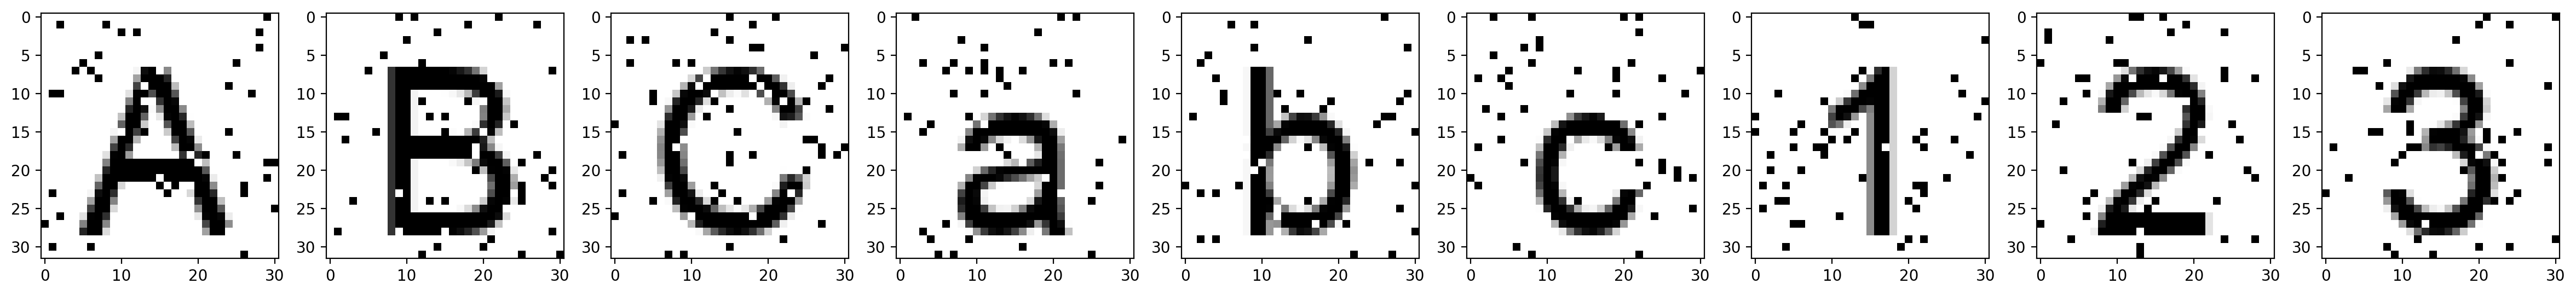
\includegraphics[width=\textwidth]{./images02/classification/example.png}
\caption{Examples of noisy images with uppercase letters, lowercase letters and numbers.
\label{fig-classification-examples}}
\end{figure}

The images had 31 pixels of width and 32 pixels of height, totaling 992 pixels per image. Each image was mapped into a 1,000 bit bitstring in which the bits were set according to the color of each pixel of the image. So, white pixels were equal to bit 0, and black pixels to bit 1. The 8 remaining bits were all set to zero. This was a bijective mapping (or one-to-one mapping), i.e., there was only one bitstring for each image, and there was only one image for each bitstring.

% TODO Add image showing the association between pixels and bits.

A total of 62 classification groups have been trained in the SDM. For each of them, it was generated a random bitstring. Thus, the groups' bitstrings were orthogonal between any two of them. There is one image for each of the 62 groups in Figure \ref{fig-classification-groups}. Notice that the SDM has never seen a single image with no noise.

\begin{figure}[!htb]
\centering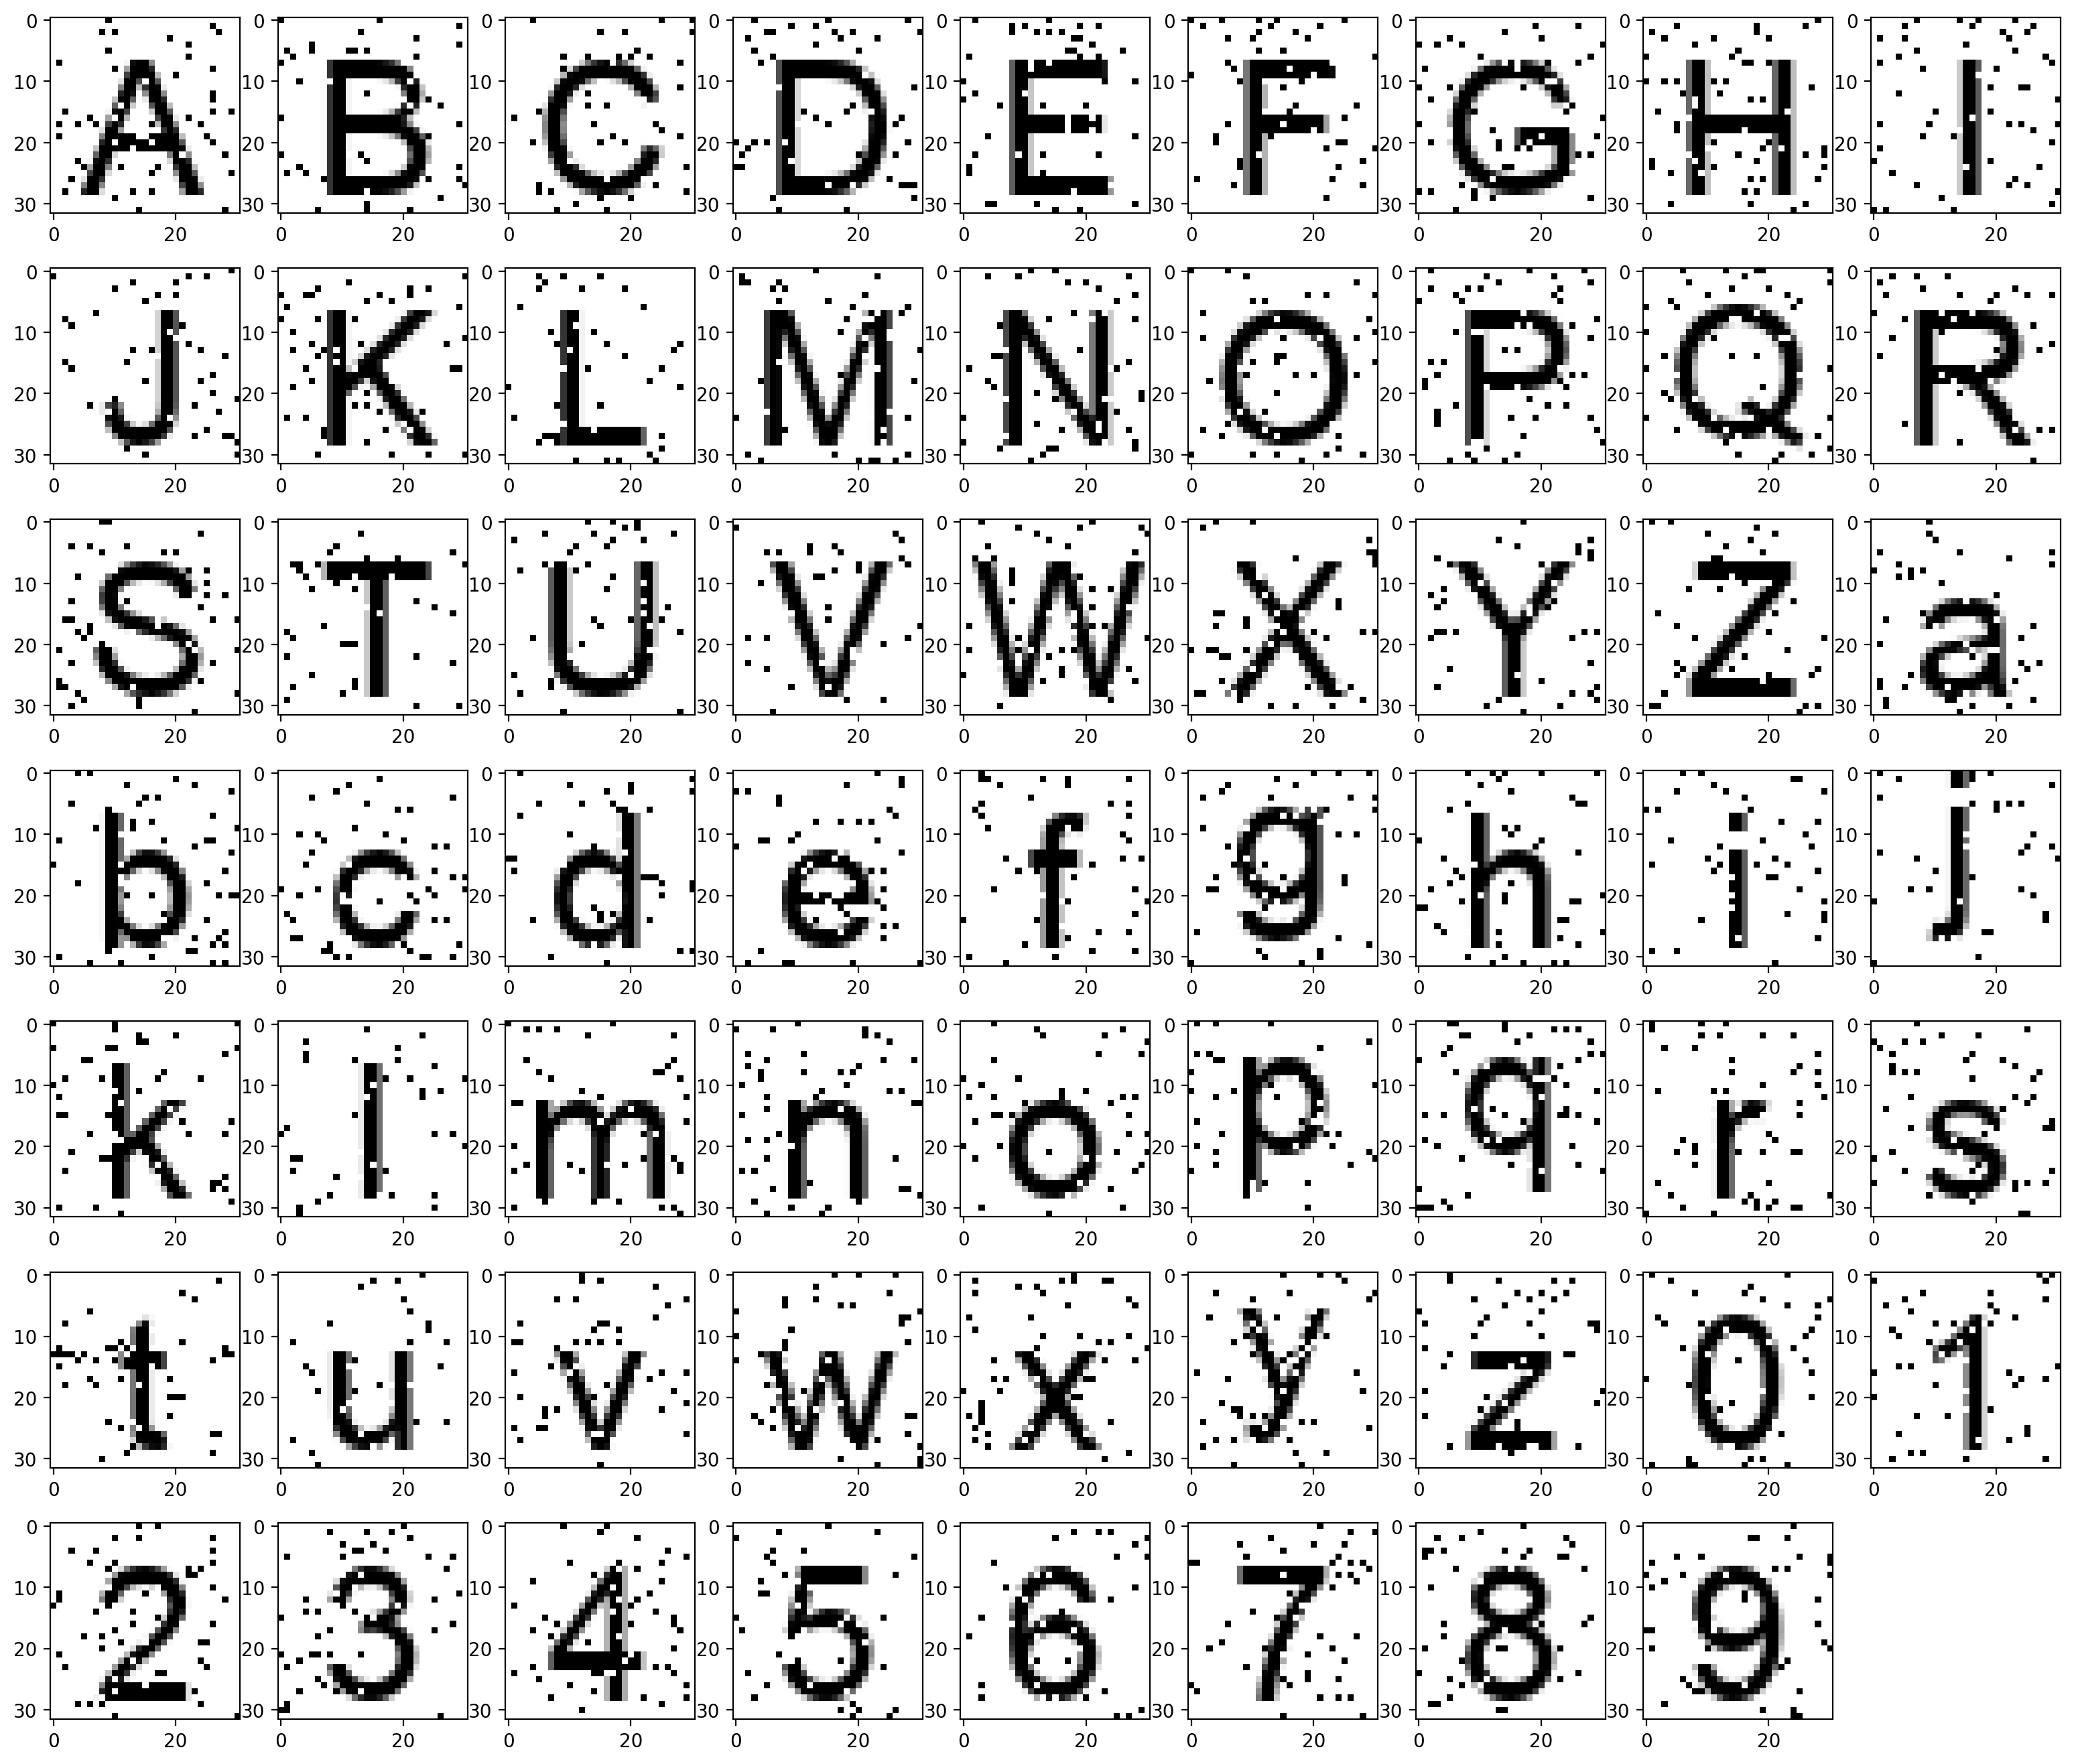
\includegraphics[width=\textwidth]{./images02/classification/groups.png}
\caption{One noisy image for each of the 62 classification groups.
\label{fig-classification-groups}}
\end{figure}

The association of images to groups was stored as sequences in SDM, as detailed by \citet{Kanerva1988} in Chapter 8. During the learning phase, the image bitstrings were stored pointing to their groups bitstrings, i.e., write(addr=bs\_image, datum=bs\_label). Thus, in order to classify an unknown image, we only had to read from its address and check which group has been found.

% TODO Add image showing the pointers.

During the learning phase, we have generated 100 noisy images for each character. The images had 5\% of noise, i.e., 5\% of their pixels have been randomly flipped. For example, see the generated images for letter A in Figure \ref{fig-classification-training-A}. Then, we have wrote the classification group bitstring into the bitstring associated to each noisy image, i.e., write(bs\_image, bs\_label). For a complete image training set, see Appendix XYZ.

\begin{figure}[!htb]
\centering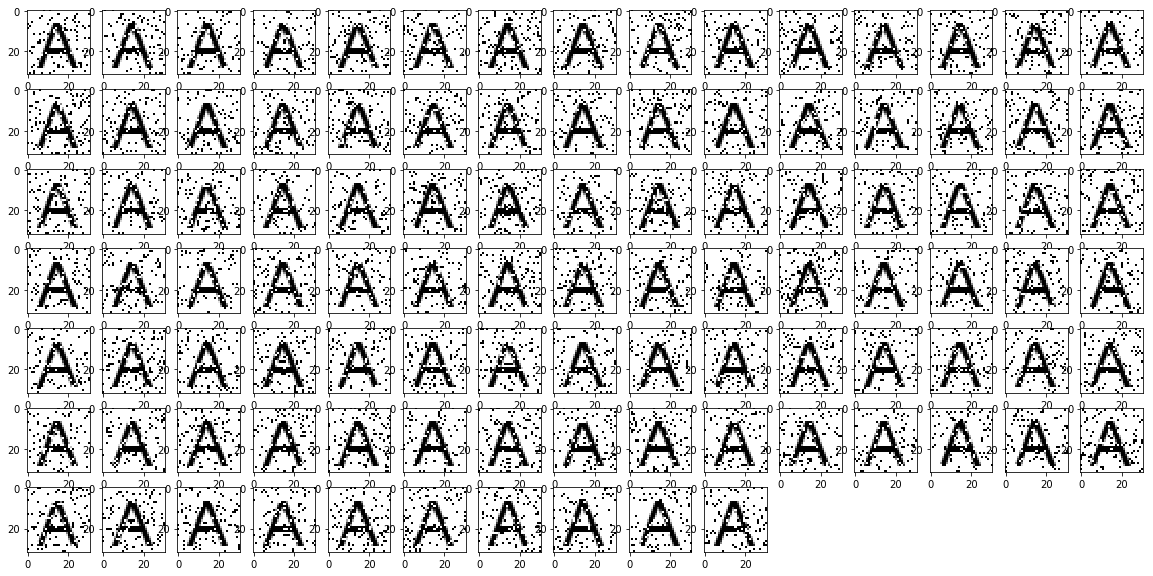
\includegraphics[width=\textwidth]{./images02/classification/trainingA.png}
\caption{100 noisy images generated to train label A.
\label{fig-classification-training-A}}
\end{figure}

Finally, we have assess the performance of our classifier. We had done it in three different scenarios: high noise (20\%), low noise (5\%) and no noise. See Figures \ref{fig-classification-noise-high} and \ref{fig-classification-no-noise} for images with 20\% noise and no noise. The low noise scenario had the same noise as the training set. For each scenario, we had classified 620 unknown images with 10 images per group.

\begin{figure}[!htb]
\centering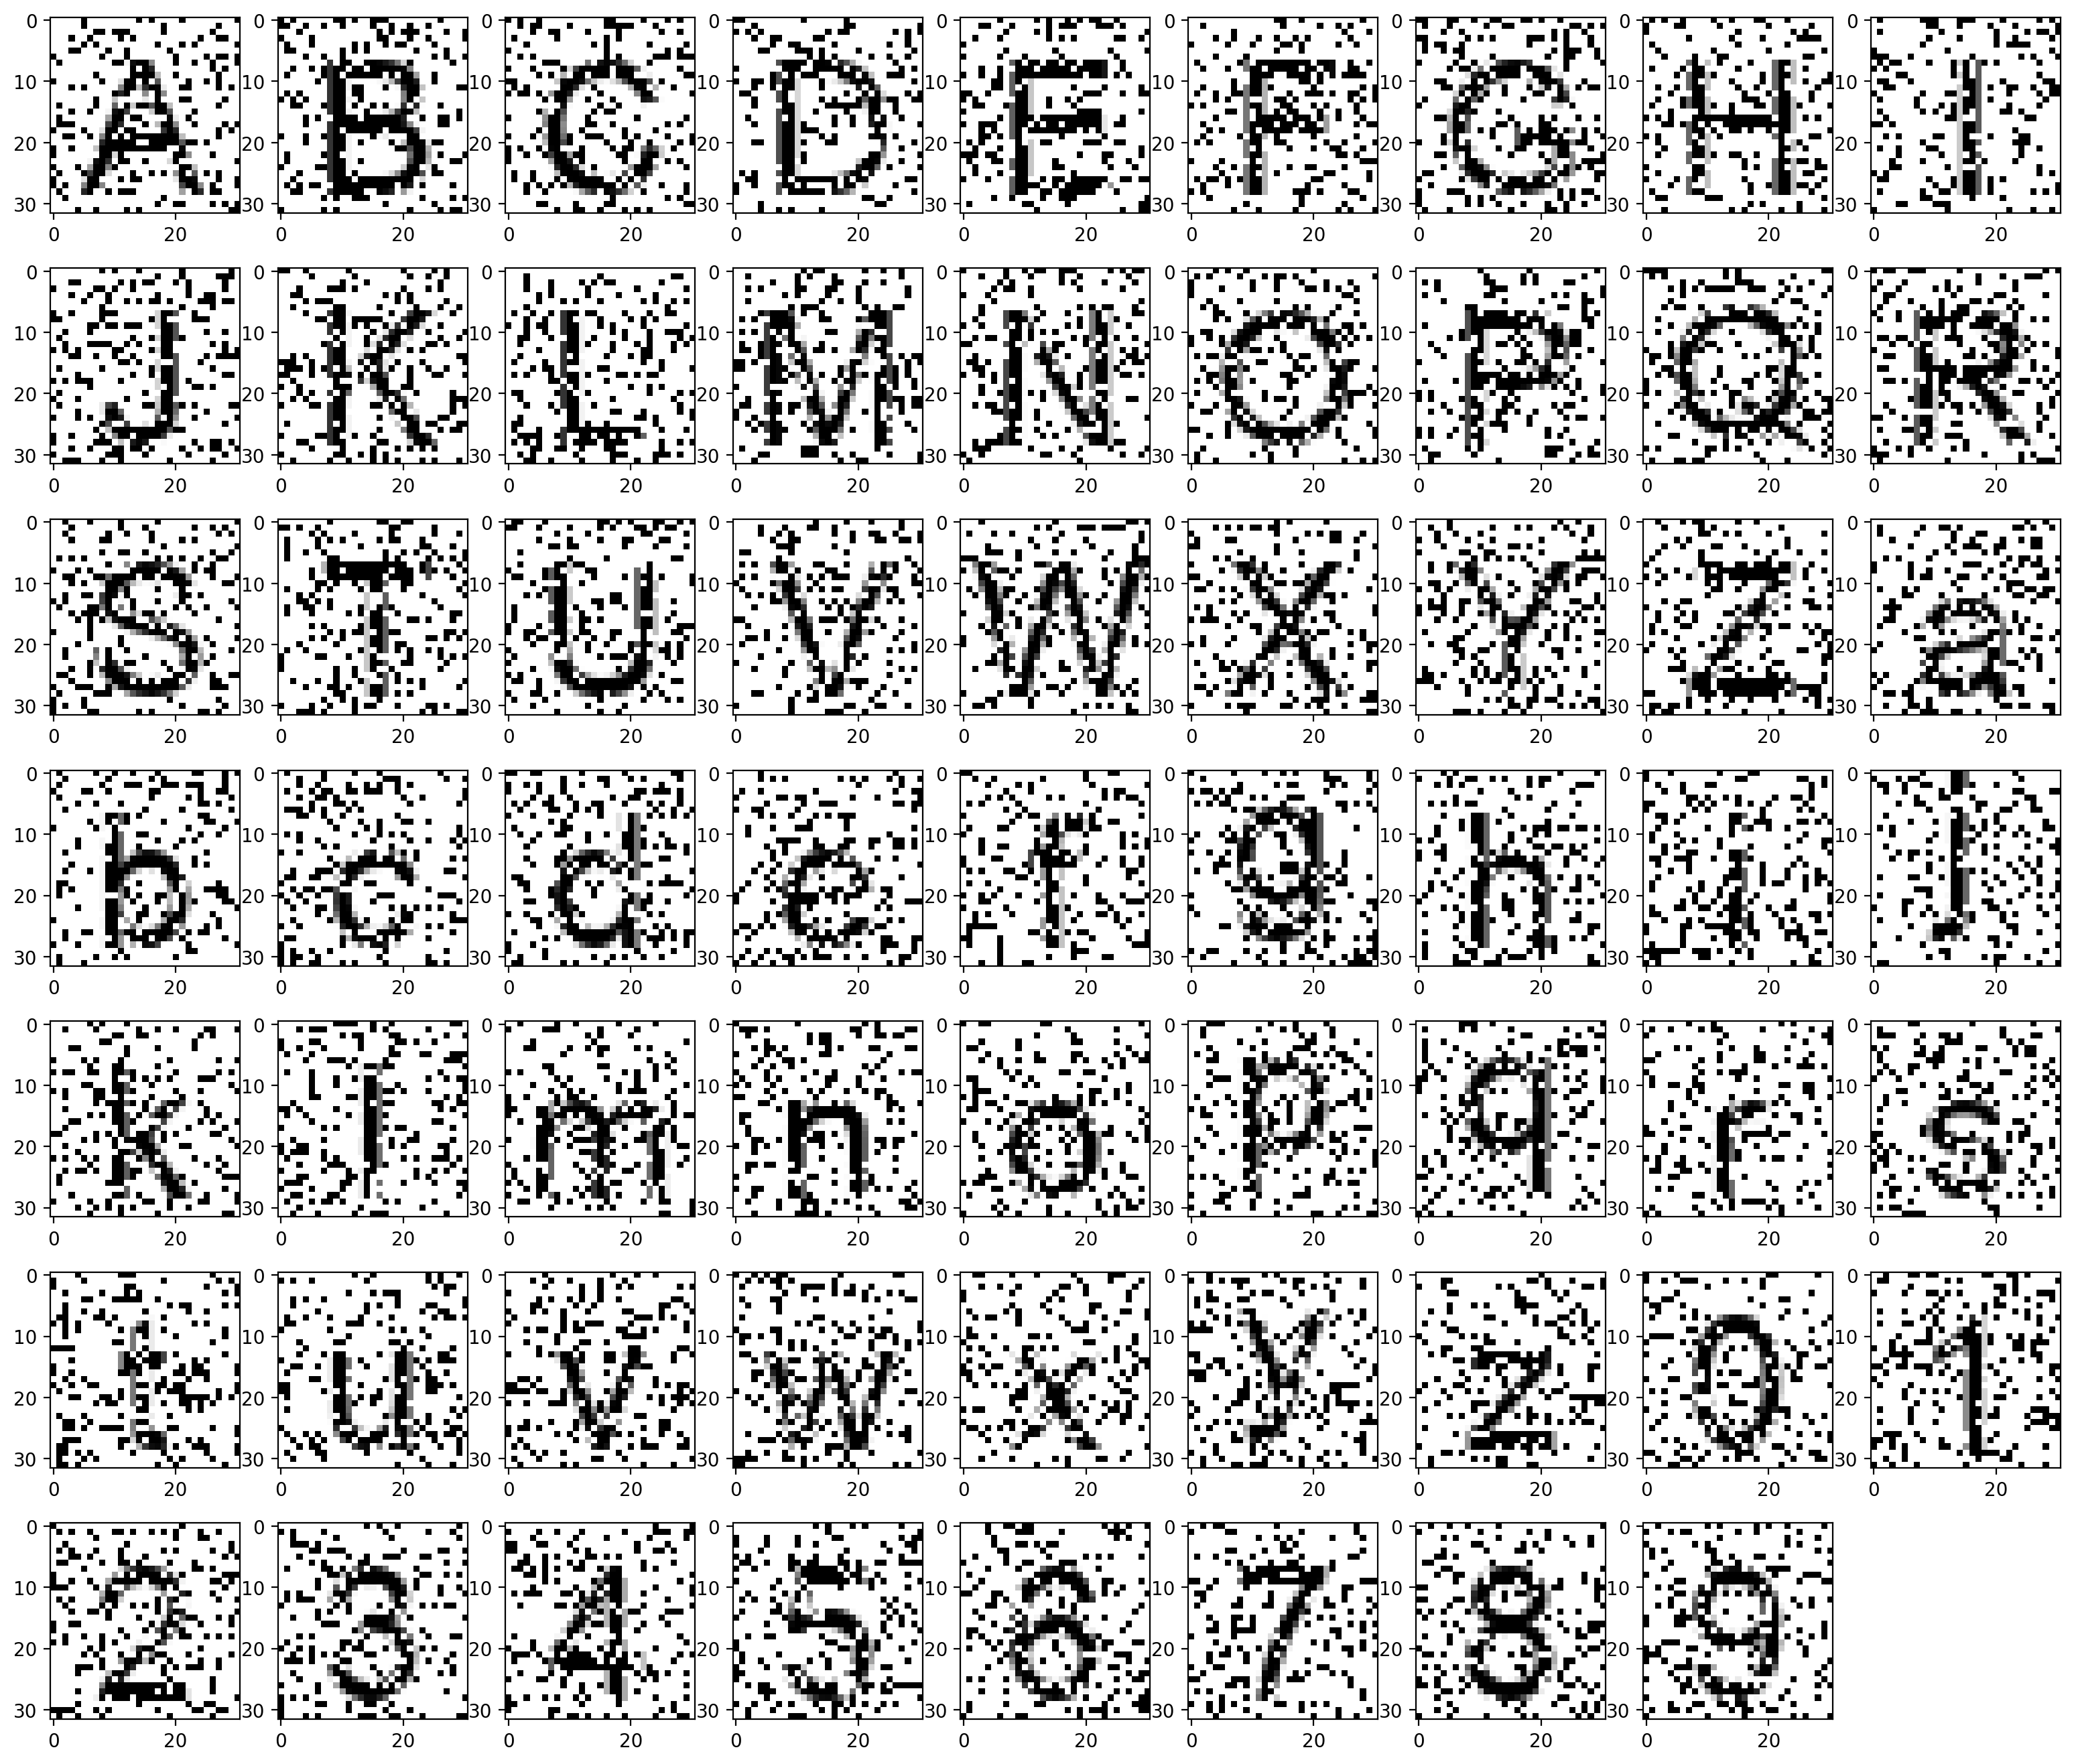
\includegraphics[width=0.75\textwidth]{./images02/classification/noise-high.png}
\caption{Images generated using a 20\% noise for the high noise scenario.
\label{fig-classification-noise-high}}
\end{figure}

\begin{figure}[!htb]
\centering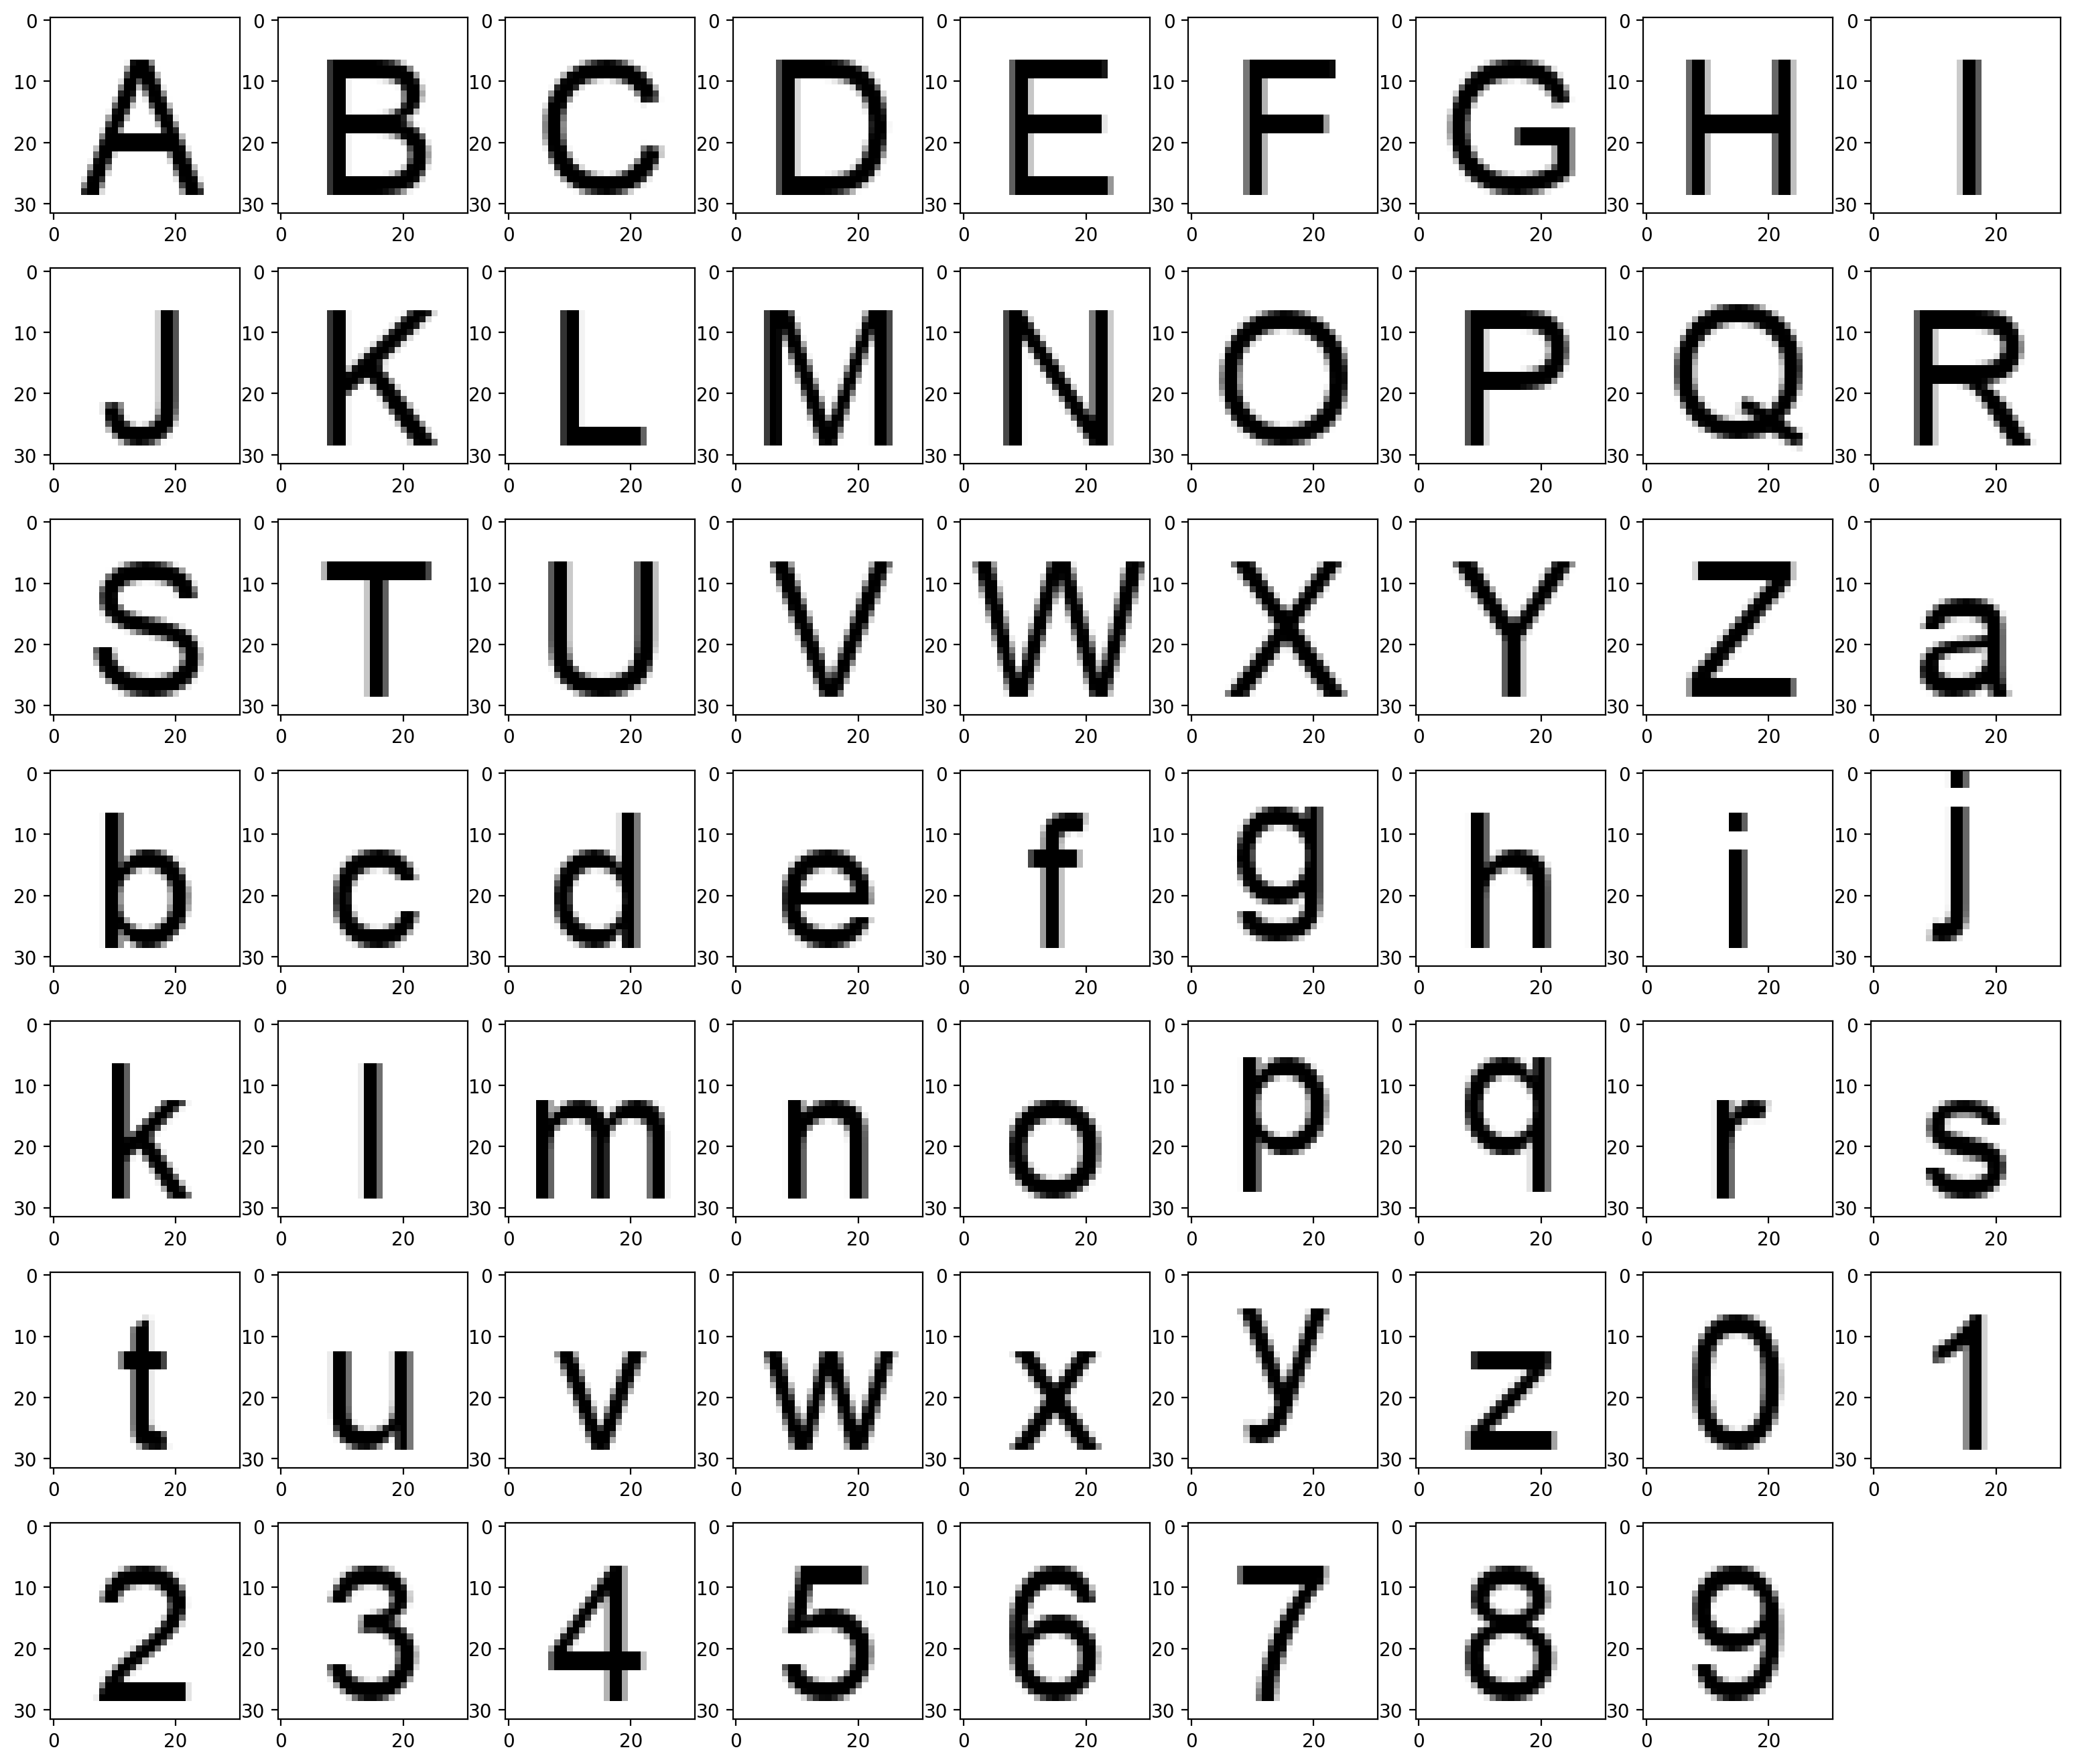
\includegraphics[width=0.75\textwidth]{./images02/classification/no-noise.png}
\caption{Images generated for the no noise scenario.
\label{fig-classification-no-noise}}
\end{figure}

The performance was calculated as the percentage of hits for each group. We did not expected the same performance for all groups because some groups become very similar to other depending on the noise level, and this similarity may even confuse a person (see Figure \ref{fig-classification-similarity}).

\begin{figure}[!htb]
  \centering
  \subfloat[``i'', ``l'', and ``r'' with 20\% noise.]{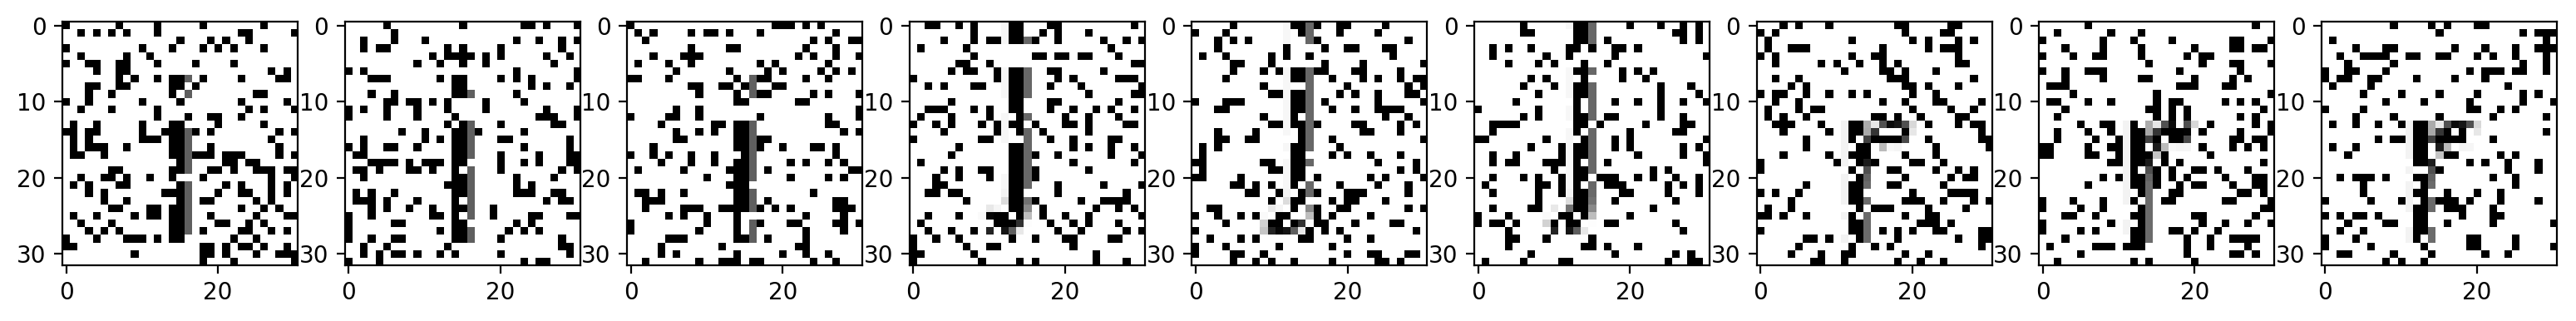
\includegraphics[width=\textwidth]{./images02/classification/ilr-high-noise.png}}

  \subfloat[``i'', ``l'', and ``r'' with 5\% noise.]{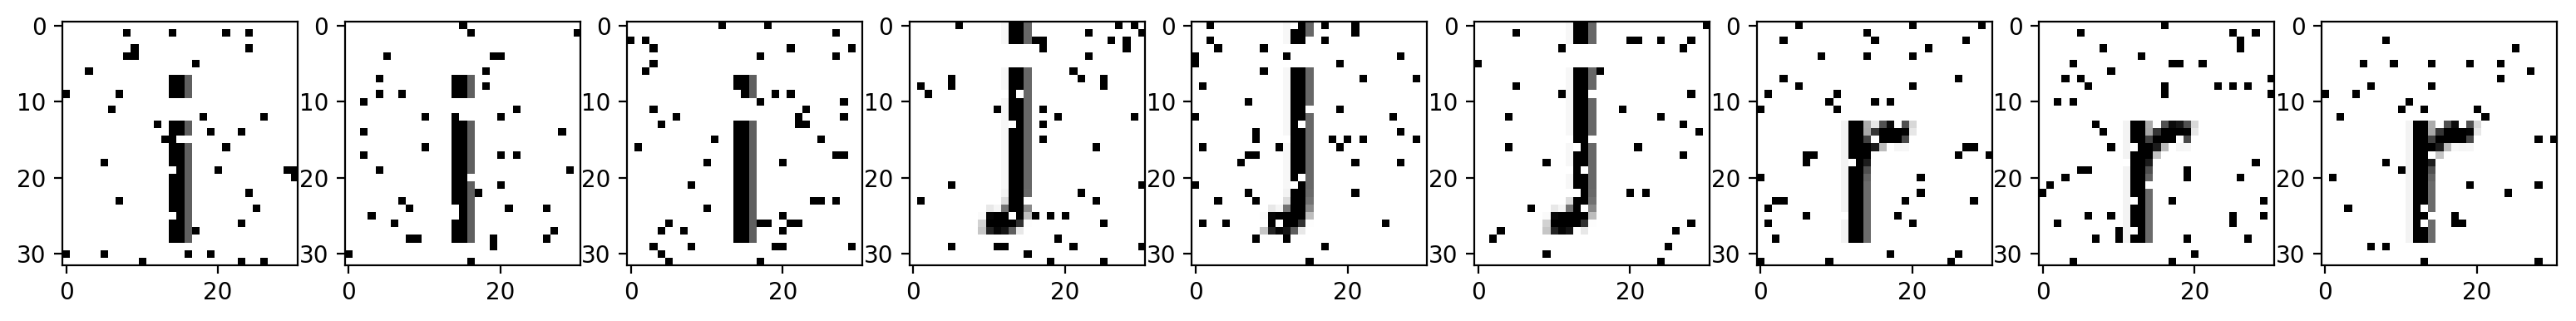
\includegraphics[width=\textwidth]{./images02/classification/ilr-low-noise.png}}

  \subfloat[``c'', ``d'', and ``o'' with 20\% noise.]{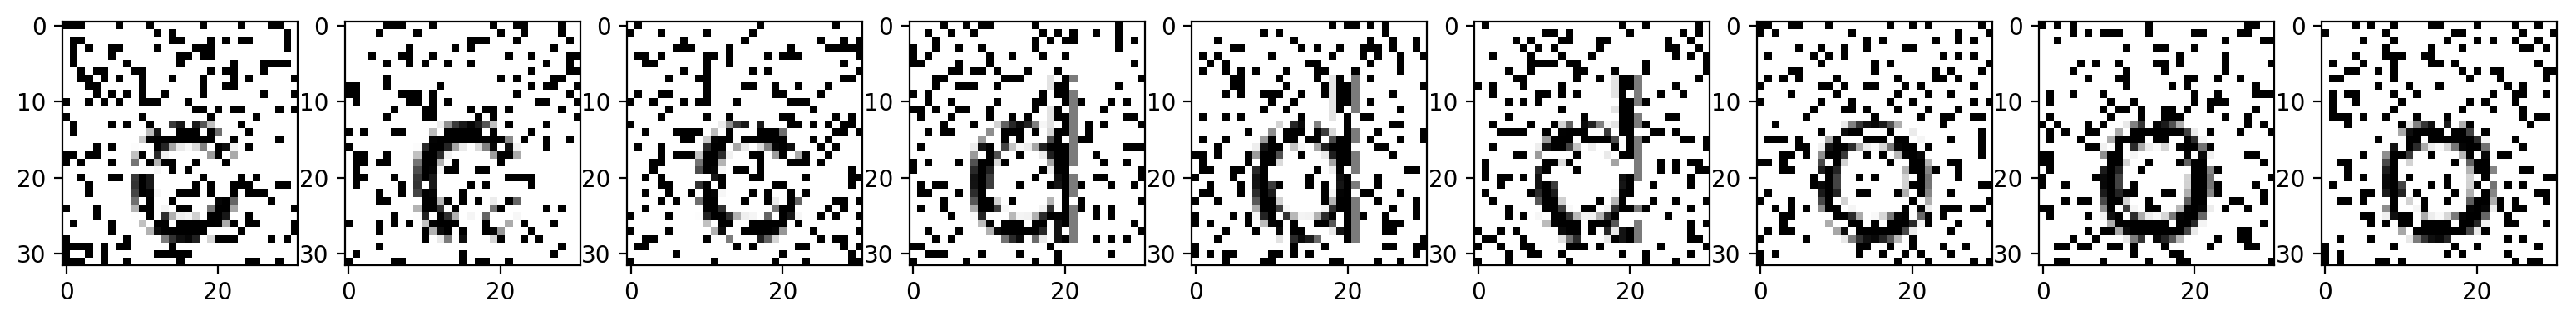
\includegraphics[width=\textwidth]{./images02/classification/cdo-high-noise.png}}

  \subfloat[``c'', ``d'', and ``o'' with 5\% noise.]{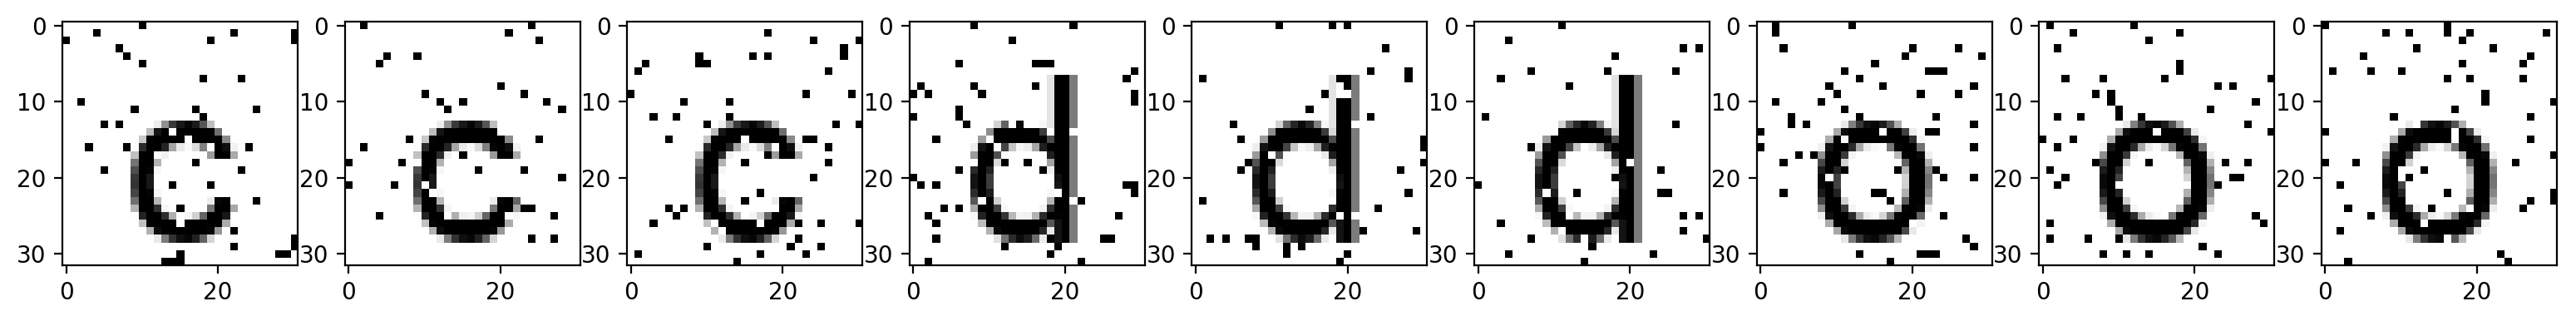
\includegraphics[width=\textwidth]{./images02/classification/cdo-low-noise.png}}

  \subfloat[``G'', ``O'', and ``Q'' with 20\% noise.]{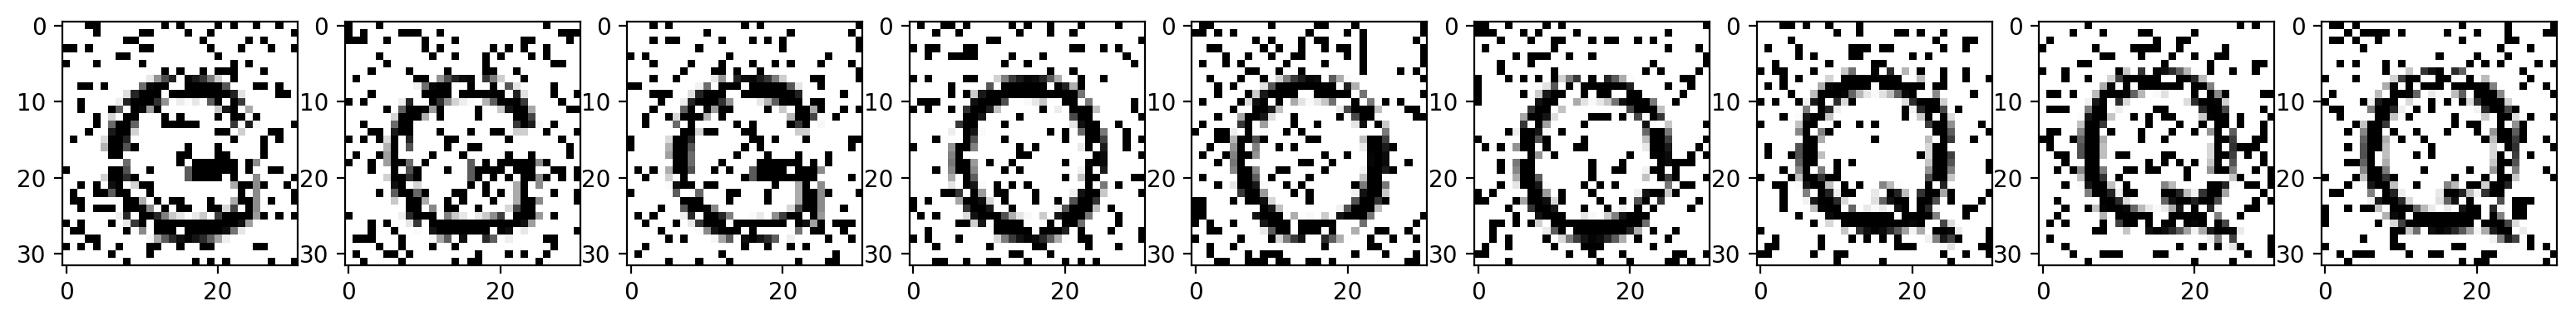
\includegraphics[width=\textwidth]{./images02/classification/GOQ-high-noise.png}}

  \subfloat[``G'', ``O'', and ``Q'' with 5\% noise.]{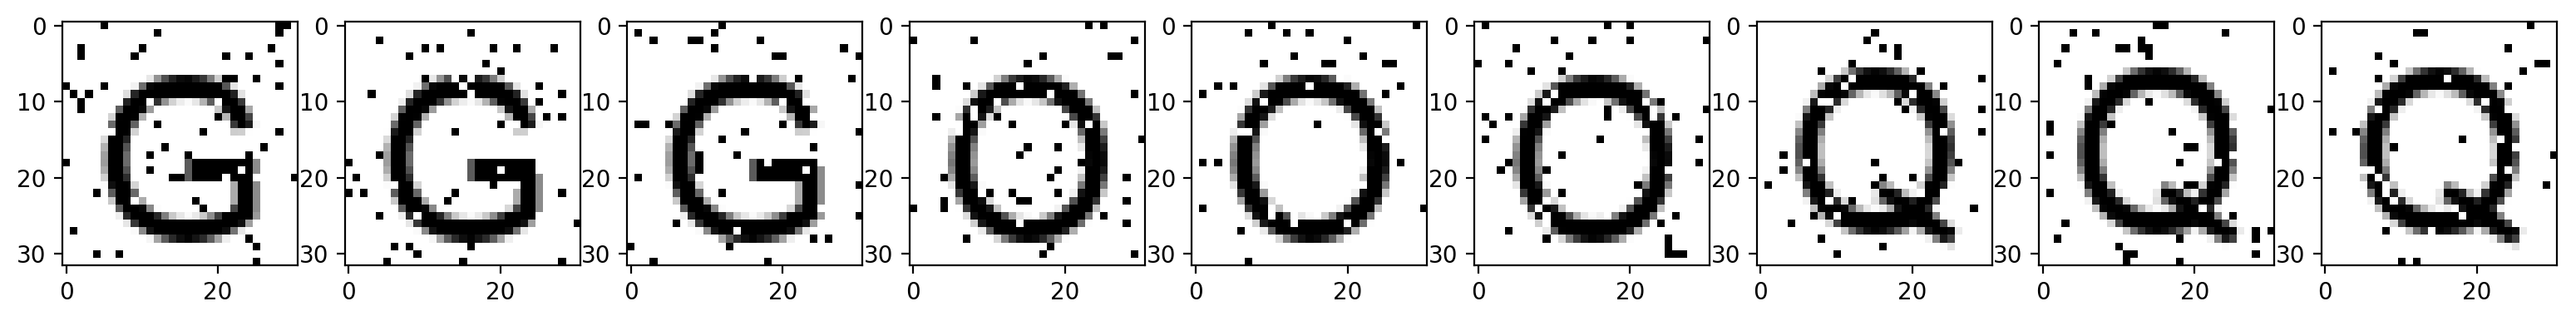
\includegraphics[width=\textwidth]{./images02/classification/GOQ-low-noise.png}}

  \caption{Images of different characters which may be confusing depending on the noise level.}
  \label{fig-classification-similarity}
\end{figure}

In the no noise scenario, the classifier has hit all characters, except letter ``l'' which was wrongly associated to the group of ``i''. We believe that it happened because the classifier had never seen an image with no noise and the difference between the images of ``l'' and ``i'' is smaller than the critical distance. So, both groups have been merged and it would converge to only one of them. In our simulation, it happened to be the group of ``i''.

In the low noise scenario, it has made few mistakes. It correctly classified all images but some from characters ``b'', ``e'', ``f'', ``l'', ``t'', and ``9''. It completely classified ``l'' images to the ``i'' group. In the other cases, it made just a few mistakes. See Figure \ref{fig-classification-low-noise-results} to check the images and their classification.

\begin{figure}[!htb]
  \centering
  \subfloat[Images from character ``b which were classified as {[b, b, b, h, b, o, b, h, b, b]}, respectively. It has made 3 misses.]{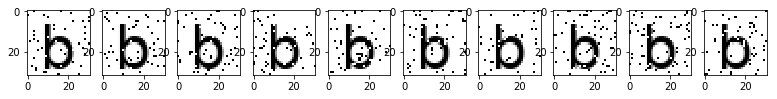
\includegraphics[width=\textwidth]{./images02/classification/low-noise-b.png}}

  \subfloat[Images from character ``e which were classified as {[e, e, e, e, e, e, e, e, o, e]}, respectively. It has made 1 miss. ]{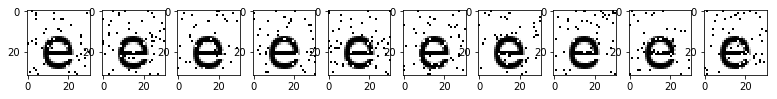
\includegraphics[width=\textwidth]{./images02/classification/low-noise-e.png}}

  \subfloat[Images from character ``f which were classified as {[i, f, f, I, I, I, f, f, f, f]}, respectively. It has made 4 misses. ]{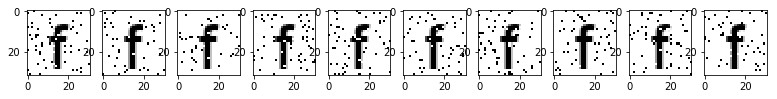
\includegraphics[width=\textwidth]{./images02/classification/low-noise-f.png}}

  \subfloat[Images from character ``l'' which were classified as {[i, i, i, i, i, i, i, i, i, i]}, respectively. It has missed them all, as if both groups have been merged. ]{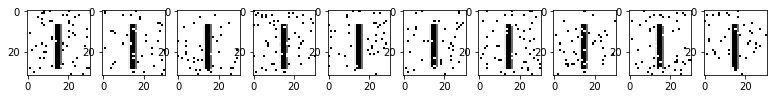
\includegraphics[width=\textwidth]{./images02/classification/low-noise-l.png}}

  \subfloat[Images from character ``t'' which were classified as {[t, t, t, t, t, t, t, i, t, t]}, respectively. It has made 1 miss. ]{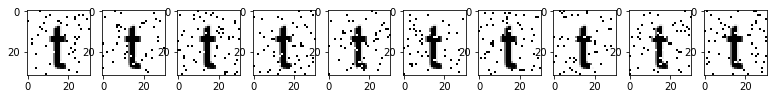
\includegraphics[width=\textwidth]{./images02/classification/low-noise-t.png}}

  \subfloat[Images from character ``9'' which were classified as {[9, 9, 0, 9, 9, 9, 0, 0, 9, 9]}, respectively. It has made 3 misses. ]{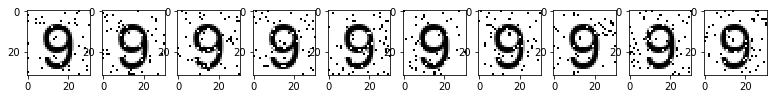
\includegraphics[width=\textwidth]{./images02/classification/low-noise-9.png}}

  \caption{Characters in the low noise scenario in which the classifier has made at least one mistake. In all the other cases, it correctly classified the images. We may notice that the groups of ``i'' and ``l'' have been completely merged by the classifier, because it cannot distinguish them, not even with no noise.}
  \label{fig-classification-low-noise-results}
\end{figure}

The high noise scenario is the most interesting, because, even in a high noise level, the classifier has hit most of the characters. It has hit all images for 44 out of 62 groups, and made at least one miss for the other 18 groups. The misses may be seen in details in Figure \ref{fig-classificiation-high-noise-misses}.

\begin{figure}[!htb]
  \centering
  \subfloat[Images from character ``B'' which were classified as {[S, B, B, B, B, B, B, B, B, B]}. It has made 1 mistake. ]{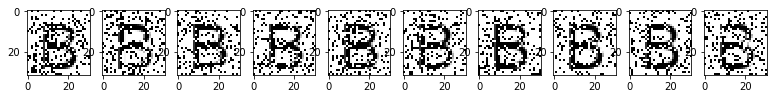
\includegraphics[width=\textwidth]{./images02/classification/high-noise-B.png}}

  \subfloat[Images from character ``O'' which were classified as {[G, G, O, O, O, O, O, O, O, O]}. It has made 2 mistakes. ]{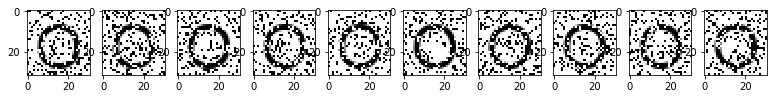
\includegraphics[width=\textwidth]{./images02/classification/high-noise-O.png}}

  \subfloat[Images from character ``T'' which were classified as {[T, T, T, T, T, I, T, T, T, T]}. It has made 1 mistake. ]{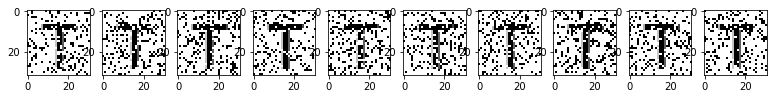
\includegraphics[width=\textwidth]{./images02/classification/high-noise-T.png}}

  \subfloat[Images from character ``Y'' which were classified as {[Y, I, Y, Y, Y, Y, Y, Y, Y, Y]}. It has made 1 mistake. ]{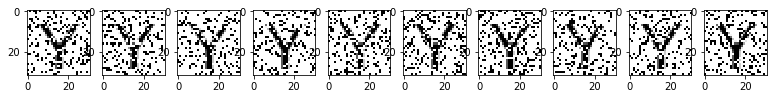
\includegraphics[width=\textwidth]{./images02/classification/high-noise-Y.png}}

  \subfloat[Images from character ``b'' which were classified as {[o, o, o, b, o, h, h, b, b, o]}. It has made 7 mistakes. ]{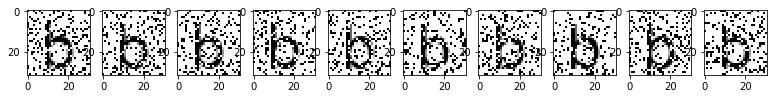
\includegraphics[width=\textwidth]{./images02/classification/high-noise-b2.png}}

  \subfloat[Images from character ``c'' which were classified as {[c, c, c, c, c, o, c, c, c, o]}. It has made 2 mistakes. ]{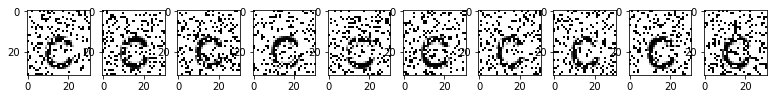
\includegraphics[width=\textwidth]{./images02/classification/high-noise-c.png}}

  \subfloat[Images from character ``e'' which were classified as {[e, o, e, o, o, o, e, o, o, e]}. It has made 6 mistakes. ]{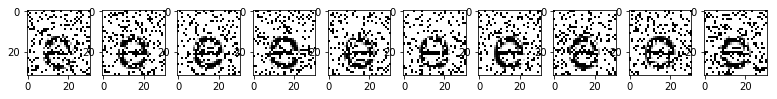
\includegraphics[width=\textwidth]{./images02/classification/high-noise-e.png}}

  \subfloat[Images from character ``f'' which were classified as {[I, I, I, I, i, I, I, I, I, I]}. It has missed them all. ]{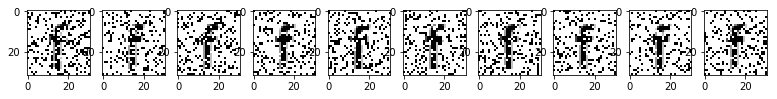
\includegraphics[width=\textwidth]{./images02/classification/high-noise-f.png}}

\end{figure}
\begin{figure}[!htb]\ContinuedFloat

  \subfloat[Images from character ``i'' which were classified as {[i, i, i, I, i, i, i, i, I, i]}. It has made 2 mistakes. ]{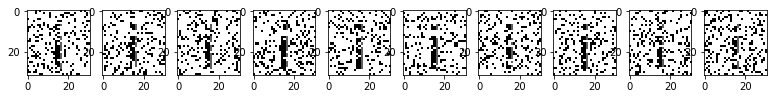
\includegraphics[width=\textwidth]{./images02/classification/high-noise-i.png}}

  \subfloat[Images from character ``j'' which were classified as {[j, j, j, I, I, j, j, j, j, I]}. It has made 3 mistakes. ]{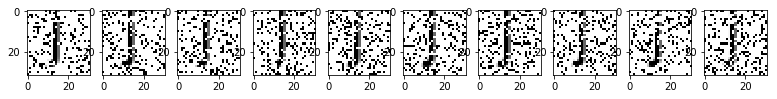
\includegraphics[width=\textwidth]{./images02/classification/high-noise-j.png}}

  \subfloat[Images from character ``l'' which were classified as {[I, i, I, I, I, I, i, I, I, i]}. It has missed them all. ]{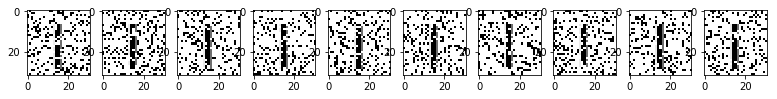
\includegraphics[width=\textwidth]{./images02/classification/high-noise-l.png}}

  \subfloat[Images from character ``n'' which were classified as {[u, n, n, n, n, n, u, u, u, h]}. It has made 5 mistakes. ]{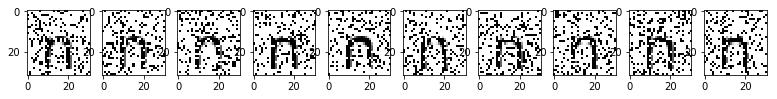
\includegraphics[width=\textwidth]{./images02/classification/high-noise-n.png}}

  \subfloat[Images from character ``q'' which were classified as {[q, q, q, q, q, q, q, q, q, g]}. It has made 1 mistake. ]{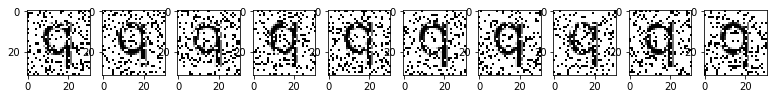
\includegraphics[width=\textwidth]{./images02/classification/high-noise-q.png}}

  \subfloat[Images from character ``t'' which were classified as {[I, r, I, i, I, i, i, i, I, i]}. It has missed them all. ]{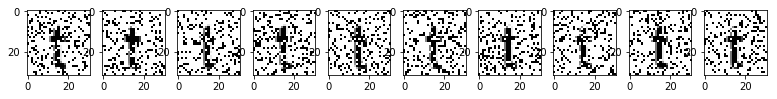
\includegraphics[width=\textwidth]{./images02/classification/high-noise-t2.png}}

  \subfloat[Images from character ``1'' which were classified as {[1, I, 1, I, 1, 1, I, I, 1, I]}. It has made 5 mistakes. ]{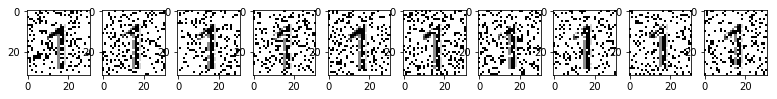
\includegraphics[width=\textwidth]{./images02/classification/high-noise-1.png}}

  \subfloat[Images from character ``7'' which were classified as {[7, 7, 7, I, 7, I, I, 7, 7, 7]}. It has made 3 mistakes. ]{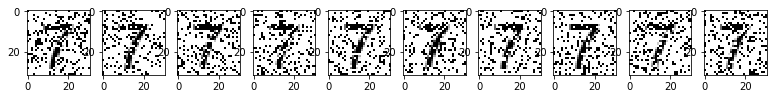
\includegraphics[width=\textwidth]{./images02/classification/high-noise-7.png}}

\end{figure}
\begin{figure}[!htb]\ContinuedFloat

  \subfloat[Images from character ``8'' which were classified as {[8, 6, 6, 6, 8, d, 8, 8, d, 6]}. It has made 6 mistakes. ]{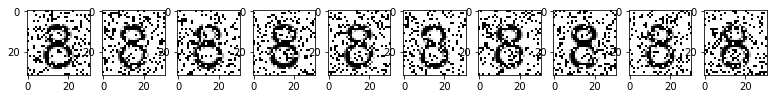
\includegraphics[width=\textwidth]{./images02/classification/high-noise-8.png}}

  \subfloat[Images from character ``9'' which were classified as {[9, 0, 6, 0, 9, 0, 0, 9, 0, 0]}. It has made 7 mistakes. ]{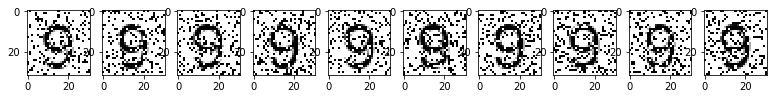
\includegraphics[width=\textwidth]{./images02/classification/high-noise-9.png}}

  \caption{Characters in the high noise scenario in which the classifier has made at least one mistake. In all the other cases, it correctly classified the images.}
  \label{fig-classification-high-noise-misses}
\end{figure}

The critical distance plays an important role in the classification error. As we have 62 groups and each have been trained with 100 images, there were 6,200 writes to the memory. When an image is being classified, it will have to converge to a group, and the convergence depends on the distance between this image and the images from the training set, i.e, in the noise level.

These results show that the SDM may be used as a supervised classification algorithm. Although we do not believe that the mapping between images and bitstrings are even close to the way human cognition deals with images, we believe the results are interesting and useful to many possible real world problems.


\section{Results (iii): Noise filtering application}




\section{Results (v): The possibility of unsupervised reinforcement learning}
